\documentclass[a4paper,11pt]{report}
\usepackage{amsmath}
\usepackage{graphicx}
\usepackage{wrapfig}
\usepackage{caption}
\usepackage{enumitem}
\usepackage{pdfpages}
\usepackage{multicol}
\usepackage[a4paper, left=3cm, right=3cm, top=3cm, bottom=3cm]{geometry}
\usepackage[ngerman]{babel}
\usepackage{hyperref}
\usepackage[x11names]{xcolor}
\usepackage{fancyhdr}
\pagestyle{fancy}
\usepackage{tikz}
\usetikzlibrary{calc}
\usepackage{titling}
\usepackage{fontspec}
\usepackage{titlesec}
\usepackage{moresize}
\usepackage{pgfplots}
\pgfplotsset{width=13cm,compat=1.9}

% font setup
\newfontfamily{\newUpperTitleFont}{Bebas Neue}
\newfontfamily{\newLowerTitleFont}{Tex Gyre Heros Bold}

% font init
\titleformat{\part}[display]{\centering\HUGE\scshape\newUpperTitleFont\color{SlateBlue4}}{\partname~\thepart}{10pt}{}
\titleformat{\chapter}{\Huge\bfseries\newUpperTitleFont\color{SlateBlue4}}{\thechapter}{1em}{}
\titleformat*{\section}{\Large\bfseries\newLowerTitleFont\color{SlateBlue3}}
\titleformat*{\subsection}{\large\bfseries\newLowerTitleFont\color{SlateBlue2}}

% hyperlink setup
\hypersetup{
    colorlinks,
    citecolor=black,
    filecolor=black,
    linkcolor=SlateBlue3,
    urlcolor=black
}

% clear Footer
\fancyfoot{}

% Header
\fancyhead[L]{Niklas Fister}
\fancyhead[C]{Kantonnschule - Mathematik}
\fancyhead[R]{\thepage}
\renewcommand{\headrulewidth}{1pt}

\fancypagestyle{plain}{
    \fancyhead[L]{Niklas Fister}
    \fancyhead[C]{Kantonnschule - Mathematik}
    \fancyhead[R]{\thepage}
    \renewcommand{\headrulewidth}{1pt}
}

% Title
\title{\Huge\textbf{Bericht Physik - Lautsprecher}}
\author{Niklas Fister}
\date{\today}

% makeing title
\begin{document}
\pagenumbering{Roman}

% pretitle
%
\includepdf[scale=1.05]{resources/pdf/Title.pdf}

% own title
\begin{titlepage}
    \centering
    \begin{tikzpicture}[remember picture, overlay]
        \draw[line width=5pt, line cap=round, color=SlateBlue1, rounded corners=5pt]($(current page.west)+(1cm, 0)$) -- ($(current page.north west)+(1cm, -1cm)$) -- ($(current page.north)+(0, -1cm)$);
        \draw[line width=5pt, line cap=round, color=SlateBlue1, rounded corners=5pt]($(current page.east)+(-1cm, 0)$) -- ($(current page.south east)+(-1cm, 1cm)$) -- ($(current page.south)+(0, 1cm)$);
    \end{tikzpicture}

    % background
    \tikz[remember picture,overlay] \node[opacity=0.3,inner sep=0pt] at (current page.center){
\includegraphics[width=\paperwidth - 4cm, height=\paperheight - 4cm]{resources/images/Mandelbrotmenge.jpg}};
    % Start Text
    \vspace{4cm}

    % the title
    {\newUpperTitleFont\thetitle\par}
    \vspace{1cm}

    % the autors
    {\theauthor\par}
    \vspace{.5cm}

    % date
    {\thedate\par}
    \vspace{5cm}

    % showcase
    %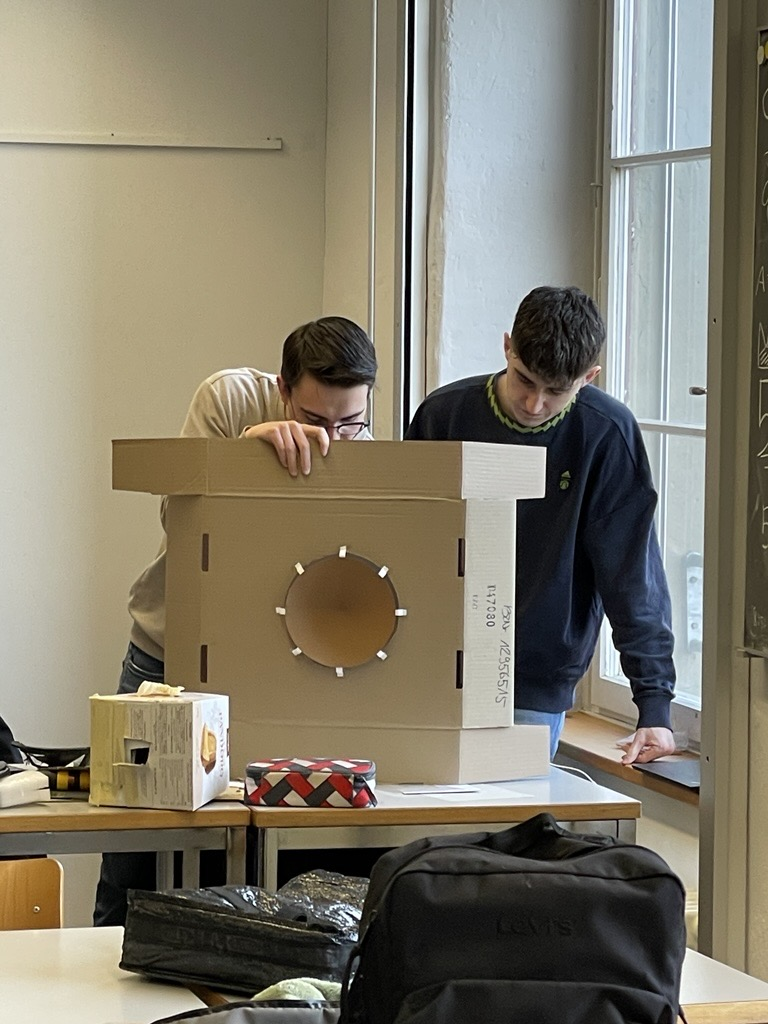
\includegraphics[width=.4\linewidth]{resources/images/Andrin_Cyrill_building.jpeg}
\end{titlepage}
\part{Analysis}
\chapter{Graphischer Zusammenhang der Analysis}
\section{Bedeutung der Ableitung}
Die Ableitung ist die Funktion, welche die Steigung einer Anderen Funktion an einem bestimmten Wert für $x$ angibt. \\
\begin{tikzpicture}
    \begin{axis}[
        axis lines = middle,
        ymin=-30,ymax=20,
        xmin=-5,xmax=10,
        xlabel=$x$,
        ylabel=$f(x)$,
    ]
    \addplot[smooth, thick, SlateBlue4, domain=-5:10]{x^3 - 3*x^2 - 9*x + 5};
    \addplot[smooth, thick, SlateBlue1, domain=-5:10]{3*x^2-6*x-9}; 
    \legend{$f(x) = x^3 - 3\cdot x^2 - 9\cdot x + 5$, $f'(x) = 3\cdot x^2 - 6\cdot x - 9$}
    \end{axis}
\end{tikzpicture}

Dies lässt sich in dieser Grafik gut erkennen. Die abgeleitete Funktion $f'(x)$ gibt die Steigung der Funktion $f(x)$ an.
\section{Graphische Darstellung des Differential}
Wie man jedoch schrittweise auf die Lösung kommt ist folgendermassen. Hierfür beginnen wir mit einer einfachen Funktion $f(x) = x^2$.
\section{Graphische Darstellung des Integral}
\end{document}